\chapter{Noosfero}

%Introdução
Neste capítulo iremos discutir o funcionamento e arquitetura do software livre Noosfero\footnote{Maiores informações em: \url{http://www.noosfero.org}}, a plataforma de redes sociais que é utilizada como núcleo do portal do Participa.br. Um dos fatores para a utilização de softwares livres no portal do Participa.br é o fato que o desenvolvimento do software ser colaborativo e todo o conteúdo criado é compartilhado, além de não haver propriedade intelectual sobre os conteúdos gerados na rede social, como foi visto na seção %CITAR DANIEL %Metodologia Participa


\section{Software Livre}

O Software livre permite aos usuários utilizarem, estudarem, modificarem e realizar a distribuição do mesmo, sem restrições e permitindo aos usuários futuros utilizarem de forma igual. %DANIEL%$$
O Software Livre garante quatro direitos básicos de liberdade aos seus usuários \footnote{Retirado de \url{http://www.gnu.org}}, entre eles:

\begin{itemize}
\item A liberdade para utilização do software de acordo com o desejo do usuário.
\item A liberdade para o entendimento do funcionamento do software, e adaptá-lo de acordo com as suas necessidades \footnote{Para satisfazer esse direito de liberdade, o código-fonte do software é um produto indispensável para o mesmo. \label{ft:codfonte}}.
\item A liberdade de redistribuição do software para qualquer pessoa.
\item A liberdade para evoluir o software, e distribuir as evoluções feitas para o público em geral, de forma a beneficiar todos os utilizadores do mesmo \footref{ft:codfonte}.
\end{itemize}

\section{Evolução de Software}

\section{Noosfero: A Plataforma Utilizada no Participa.br}
%Contexto
O Noosfero é uma plataforma livre para criação de redes sociais, que está disponível sob licença AGPL\footnote{Licença de software GNU Affero General Public License} V3. O Noosfero tem como objetivo permitir a criação de uma rede social por parte de um usuário, onde o mesmo pode modificá-lo e personizá-lo de acordo com suas necessidades. No entanto o Noosfero também pode ser adpatado para ser utilizado como um Sistema de Gerenciamento de Conteúdo (CMS), ou até mesmo funcionando em portais de economia solidária.

O Noosfero foi criado pela Colivre\footnote{Maiores Informações em: \url{http://www.coolivre.coop.br}} (Cooperativa de tecnologias livres), uma cooperativa sediada em Salvador/BA. Essa cooperativa trabalha exclusivamente com softwares livres, dentre eles, manutenção de redes sociais que utilizam o Noosfero, sites em geral, intranets com Wiki, capacitação de usuários, consultorias, entre outros. Atualmente os desenvolvedores da Colivre mantém o repositório do Noosfero, isto é, eles são responsáveis por revisar os códigos que são enviados pela comunidade e integram ao código do Noosfero.

O Noosfero é escrito na linguagem de programação \textit{Ruby} versão 1.9 (discutido na seção \ref{sec:linguagemruby} e utiliza framework para aplicações web \textit{Ruby on Rails} versão 3.2 (mais detalhes na seção \ref{sub:frameworkrails}. Utiliza também os padrões arquiteturais de software \textit{Model-View-Controller} (MVC), que será discutido na seção \ref{sub:arquiteturamvc} e o padrão básico de plugins, discutido na seção \ref{sub:arquiteturaplugin}. 

\section{A Arquitetura de Funcionamento do Noosfero}

Como visto em Fowler (2005), a definição do termo arquitetura em relação a software é bastante confusa e contraditória. Vários autores não concordam sobre uma definição especifica e definem de maneira errônea, logo é necessário se chegar a um ``consenso ´´. Segundo Garlan and Perry (1995), uma arquitetura de software é definido como a estrutura de todos componentes que compõe aquele software, assim como suas relações e especificações que vão desde a concepção, desenvolvimento e evolução durante ao longo do ciclo de vida. Já para (Bass, Clements, and Kazman, 1998), a arquitetura de software é definida pela estrutura ou estruturas utilizadas pelo sistema, que são os componentes que fazem parte do software, assim como suas relações, além das propriedades que são visíveis externamente e as relações desses componentes.

Detalhar alguns padrões arquiteturais utilizado no Noosfero é importante, já que o entendimento do sistema será maior sobre os elementos essenciais e suas relações, deixando de lado detalhes desnecessários e irrelevantes. (Software Systems Architecture, Addison Wesley). Sendo assim, o entendimento da arquitetura de funcionamento do Noosfero é um dos passos iniciais para evolução do Participa.br, alcançando os objetivos propostos nesse trabalho.



\subsection{A Linguagem de Programação \textit{Ruby}}
\label{sec:linguagemruby}

Uma das vantagens da linguagem \textit{Ruby} é o fato dele possuir gemas (\textit{gems})

\subsection{Extendendo o \textit{Ruby} para Aplicações Web Através do \textit{Framework Rails}}
\label{sub:frameworkrails}

O \textit{Rails} é um arcabouço de desenvolvimento web escrito na linguagem \textit{Ruby}, ele foi criado no ano de 2004 por David Heinemeier Hansson. O Rails possui como uma das suas principais premissas facilitar o desenvolvimento de aplicativos, isto é, com o Rails é possível criar uma aplicação completa com conexão com banco de dados em apenas 10 minutos. O rails utiliza vários princípios em sua arquitetura para orientar desenvolvimento do ´´modo certo`` ou ´´Rails way``, possibilitando o programador focar o seu desenvolvimento no problema do cliente, deixando a parte da estrutura da aplicação por conta do arcabouço. %VINICIM

O arcabouço \textit{Ruby on Rails} influencia em maior produtividade graças a conceitos como:

\begin{itemize}
\item DRY - \textit{Don’t Repeat Yourself} - É um conceito que evita a duplicação de código fonte, onde propõe que um mesmo trecho de código deve possuir representação único no sistema. Isso garante que uma alteração no software seja realizada em um único local no código, evitando  \textit{´´bad smells``} como código duplicado e facilitando a manutenibilidade do sistema.
\item Paradigma de Programação Orientado à Convenção \textit{Convention Over Configuration} - Esse paradigma facilita o desenvolvimento de software, pois diminui o tempo que o programador gasta integrando serviços e configurando todo os seus módulos (banco de dados, ferramentas para teste, entre outros). Nesse paradigma o desenvolvedor pode se preocupar com a lógica de negócio, deixando a lógica de aplicação à cargo do suporte orientado à convenção sobre configuração.
\item REST \textit{Representaional State Transfer.} É um estilo arquitetural para aplicações web. Ele propõe princípios (não exclusivos ao REST) que definem
como \textit{Web Standards} como HTTP e URIs devem ser usados.
\item Múltiplos ambientes - \textit{No Rails}, cada aplicativo possui três ambientes. Um desses ambientes é voltado para o desenvolvimento do software em si, outro para testar o software através de testes e mais uma utilizada para o software entrar em produção. Cada um desses ambientes possuem comportamentos quase iguais, no entanto, cada um utiliza um banco de dados diferente.
\end{itemize}

Devido ao fato do Noosfero ter sido desenvolvido em cima do arcabouço \textit{Ruby on Rails}, sua arquitetura é altamente ligada a arquitetura do mesmo. Essa arquitetura é ilustrada pela figura \ref{fig:arquiteturaror}.

\graphicspath{{figuras/}}
\begin{figure}[H]
\centering
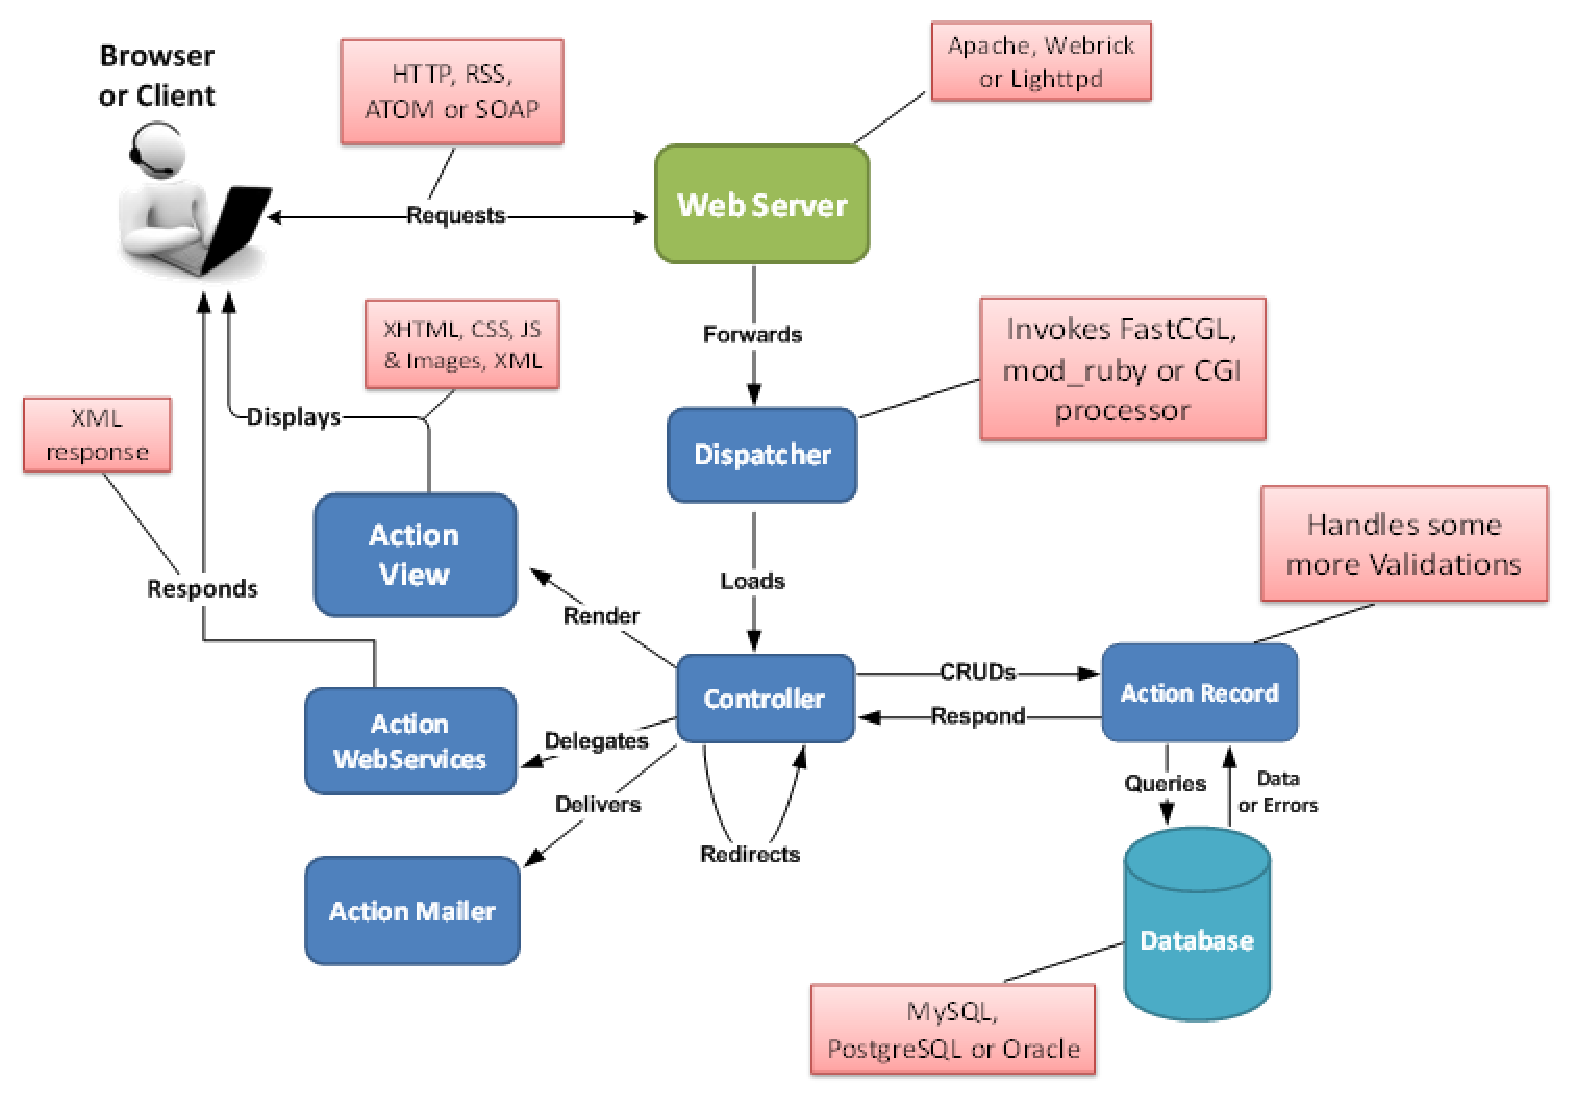
\includegraphics[width=0.7\textwidth]{rails-overview}
\caption{Arquitetura de funcionamento do \textit{Ruby On Rails}. Extraído de \cite{mejia2011rails}}
\label{fig:arquiteturaror}
\end{figure}

Essas tecnologias foram escolhidas pois a linguagem \textit{Ruby} possui uma sintaxe simples, que facilita a manutenibilidade do sistema, característica importante em projetos de software livre que tendem a atrair colaboradores externos a equipe. E o \textit{Rails} como visto acima, possui conceitos que auxiliam em sua produtividade. %CITAR PRMM

\subsection{Arquitetura MVC}
\label{sub:arquiteturamvc}

O padrão arquitetural MVC (\textit{\textbf{M}odel \textbf{V}iew \textbf{C}ontroller})foi desenvolvido por Trygve Reenskaug nos anos 70. Como dito em Fowler(2005), o MVC tem exercido grande influência nos projetos de interface com o usuário, isso inclui o \textit{Ruby On Rails}.

O arcabouço para aplicações web \textit{Ruby On Rails} apoia a utilização  MVC, que sugere que o software deve ser dividido em componentes, separando em camadas de persistência, logica e interface. Isso torna o desenvolvimento do software muito mais organizado, claro e enxuto, facilitando a manutenção e evolução do sistema e com mantém a segurança do software em fases posteriores do seu desenvolvimento\cite{} (SILVA, 2012). Porém, o baixo acoplamento e alta coesão de um software, com módulos responsáveis só é garantido se houver uma organização do sistema em camadas, garantindo assim a escalabilidade, eficiência e a reusabilidade. Na figura \ref{fig:arquiteturamvc}, temos a arquitetura de funcionamento da arquitetura MVC.

\graphicspath{{figuras/}}
\begin{figure}[H]
\centering
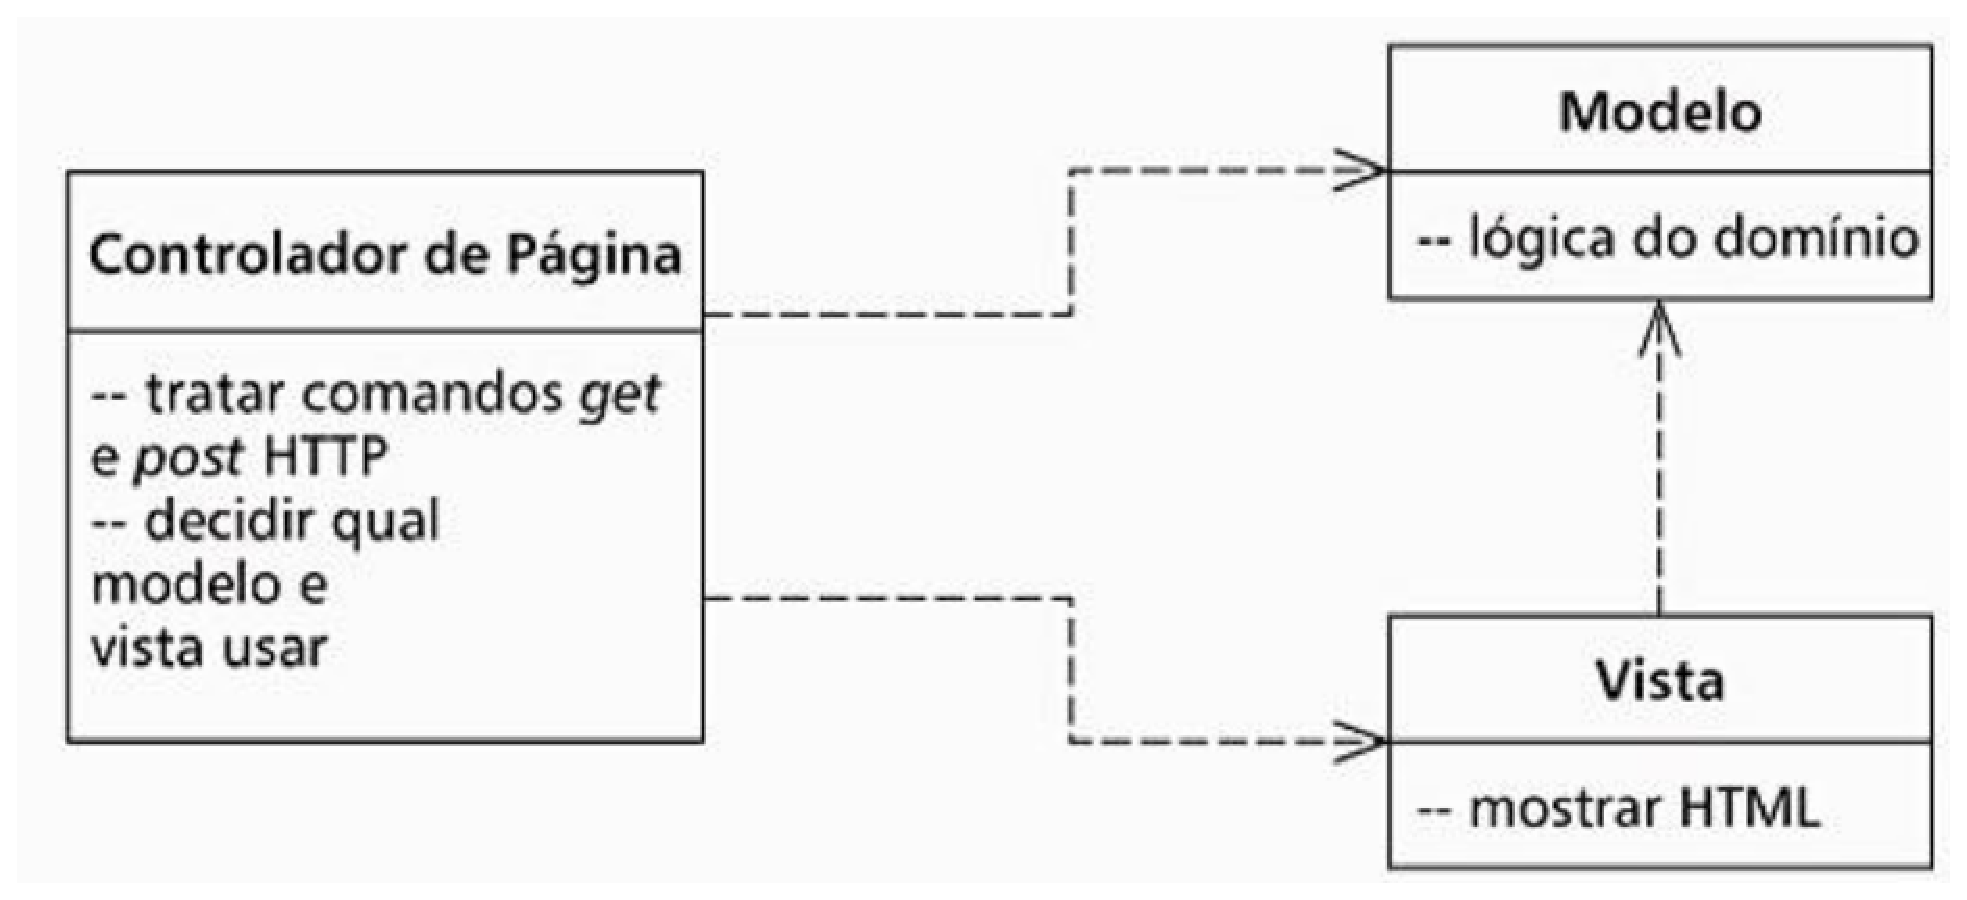
\includegraphics[width=0.6\textwidth]{funcionamentomvc}
\caption[Funcionamento do \textit{Model View Controller}]{Funcionamento do \textit{Model View Controller}. Extraído de FOWLER}
\label{fig:arquiteturamvc}
\end{figure}

Nessa visão em camadas, (i) o modelo (\textit{model}) possui informações sobre a regra de negócio, comportamentos e dados que não são utilizados na interface de usuário, (ii) a vista (\textit{view}) é composta pela saída que é vista pelo usuário do sistema, por exemplo, uma página HTML, (iii) o controlador (\textit{controller}) é responsável por receber as requisições (entradas) enviadas pelo cliente e decide qual o modelo que deve ser utilizado por aquela requisição e faz com que a vista seja renderizada para o usuário. Essa combinação entre vista e controladora é chamada de interface de usuário (Fowler 2005).

Como dito acima, a implementação desse padrão arquitetural em camadas no Noosfero é inerentes ao arcabouço utilizado.

\subsection{Plugins: Uma Arquitetura Extensível no Noosfero}
\label{sub:arquiteturaplugin}
%Arquitetura de plugins do Noosfero
O Noosfero também utiliza uma arquitetura extensível através do uso de plugins. Essa arquitetura é interessante, pois no Noosfero existem múltiplos ambientes que requerem comportamentos que tenham implementações diferentes %(FOWLER). 

%%Software Systems Architecture, Addison Wesley  
Essa arquitetura encoraja a criação de um software modular, ou seja, a criação de módulos específicos para cada função diminuindo o acoplamento, aumentando a coesão e definindo bem as responsabilidades de cada módulo.  
%
Uma das grandes vantagens em se criar uma aplicação com arquitetura extensível através de plugins, é o fato de o desenvolvedor criarem novas funcionalidades sem ter acesso ao código fonte do software, apenas é necessário somente a API que é fornecida pelo fabricante do software. Apesar disso no Noosfero os plugins são mantidos acoplados com o código principal (núcleo), isso ajuda no auxílio no controle de qualidade do ambiente. Pensando nisso os plugins devem ter testes automatizados. Quando houver a necessidade de alterar o código do Noosfero, os testes dos plugins são executados para verificar se as mudanças não afetaram seu funcionamento~\footnote{\url{http://noosfero.org/Development/Plugins}}.
%
O funcionamento dos plugins é inspirado no paradigma de orientação a eventos, onde núcleo do Noosfero dispara um evento durante a execução de alguma função, e os plugins interessados nesse evento vão sobrescrever o método do core do Noosfero tratando o evento de acordo com sua implementação. Os eventos que são disparados pelo Noosfero são chamados de “hotspots”.

\subsection{Testes: Mantendo a Qualidade do Código do Noosfero}
\label{sub:arquiteturatestes}